\subsection{Abhängigkeit der Energie der Elektronen von der Lichtfrequenz}
Die Messwerte des Photostroms I und der Gegenspannung U sind in Tabelle \ref{tab:v405}, \ref{tab:v436}, \ref{tab:g492}, \ref{tab:g546} und \ref{tab:o578} notiert.
$\sqrt{I}$ ist in den Abbildungen \ref{fig:v405}, \ref{fig:v436}, \ref{fig:g492}, \ref{fig:g546} und \ref{fig:o578} für verschiedene Wellenlängen gegen $U$ aufgetragen.
Die lineare Regression der Form $y=ax+b$ wird jeweils mit Python erstellt.
Die Grenzspannung $U_g=x$ wird als Nullstelle berechnet mit
\begin{equation*}
0=ax+b \Leftrightarrow x=-\frac{b}{a}.
\end{equation*}
Analog erfolgt die Rechnung für die weiteren Wellenlängen.
\begin{table}[h!]
  \centering
  \caption{Photostrom $I$ in Abhängigkeit von der Bremsspannung $U$ für $\lambda=\SI{405}{nm}$}
  \label{tab:v405}
  \begin{tabular}{c c c}
    \toprule
      U/V & I/nA  & $\sqrt{I}$/$\sqrt{nA}$  \\
    \midrule
      0,001 & 0,40 & 0,633 \\
      0,142 & 0,35 & 0,592 \\
      0,100 & 0,30 & 0,548 \\
      0,223 & 0,27 & 0,520 \\
      0,355 & 0,20 & 0,447 \\
      0,354 & 0,14 & 0,374 \\
      0,444 & 0,10 & 0,316 \\
      0,691 & 0,07 & 0,265 \\
      0,686 & 0,05 & 0,224 \\
      0,905 & 0,03 & 0,173 \\

    \bottomrule
  \end{tabular}
\end{table}

\FloatBarrier
\begin{figure}[h!]
  \centering
  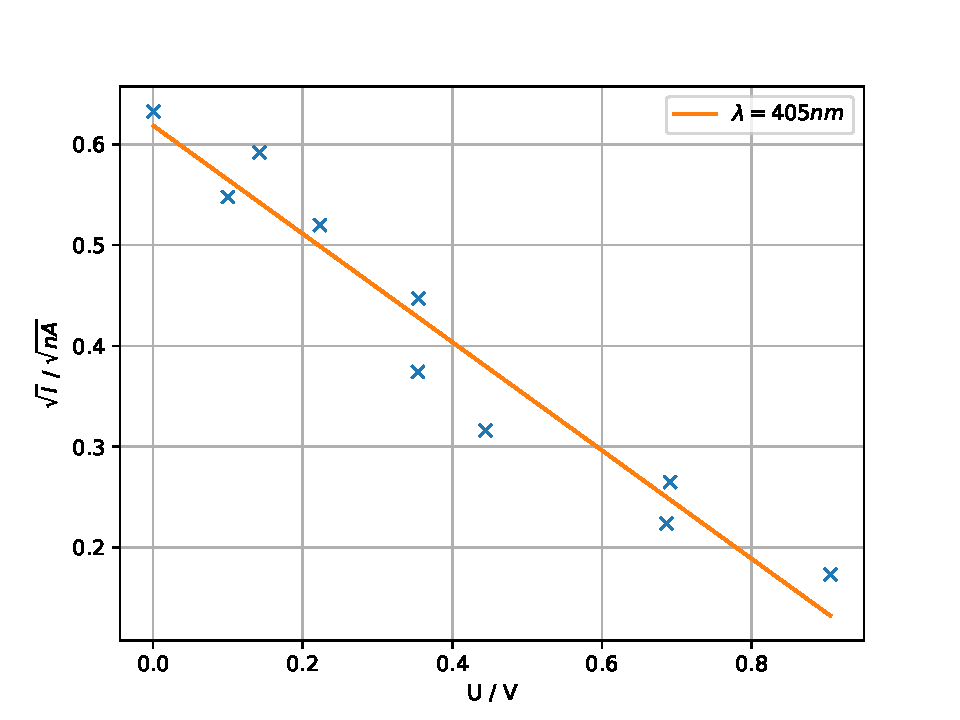
\includegraphics[width=\textwidth]{Violett405.pdf}
  \caption{Photostrom $I$ gegen Bremsspannung $U$ für $\lambda=405nm$ (Violett)}
  \label{fig:v405}
\end{figure}
\FloatBarrier
\begin{align*}
  a &= (-1,699 \pm 2,168 \cdot 10^{-7}) 10^{-5}\si{\frac{\sqrt{A}}{V}}\\
  b &= (1,956 \pm 4,976 \cdot 10^{-8}) 10^{-5} \si{\sqrt{A}}\\
  -\frac{b}{a} &= \SI{1.151}{V}
\end{align*}
\FloatBarrier
\begin{table}[h!]
  \centering
  \caption{Photostrom $I$ in Abhängigkeit von der Bremsspannung $U$ für $\lambda=\SI{436}{nm}$}
  \label{tab:v436}
  \begin{tabular}{c c c}
    \toprule
      U/V & I/nA  & $\sqrt{I}$/$\sqrt{nA}$ \\
    \midrule
      0,001 & 1,2  & 1,095 \\
      0,061 & 1,0  & 1,000 \\
      0,111 & 0,9  & 0,949 \\
      0,159 & 0,81 & 0,900 \\
      0,231 & 0,69 & 0,831 \\
      0,295 & 0,61 & 0,781 \\
      0,356 & 0,5  & 0,707 \\
      0,422 & 0,4  & 0,632 \\
      0,499 & 0,29 & 0,538 \\
      0,577 & 0,2  & 0,447 \\
      0,702 & 0,1  & 0,316 \\

    \bottomrule
  \end{tabular}
\end{table}

\FloatBarrier
\begin{figure}[h!]
  \centering
  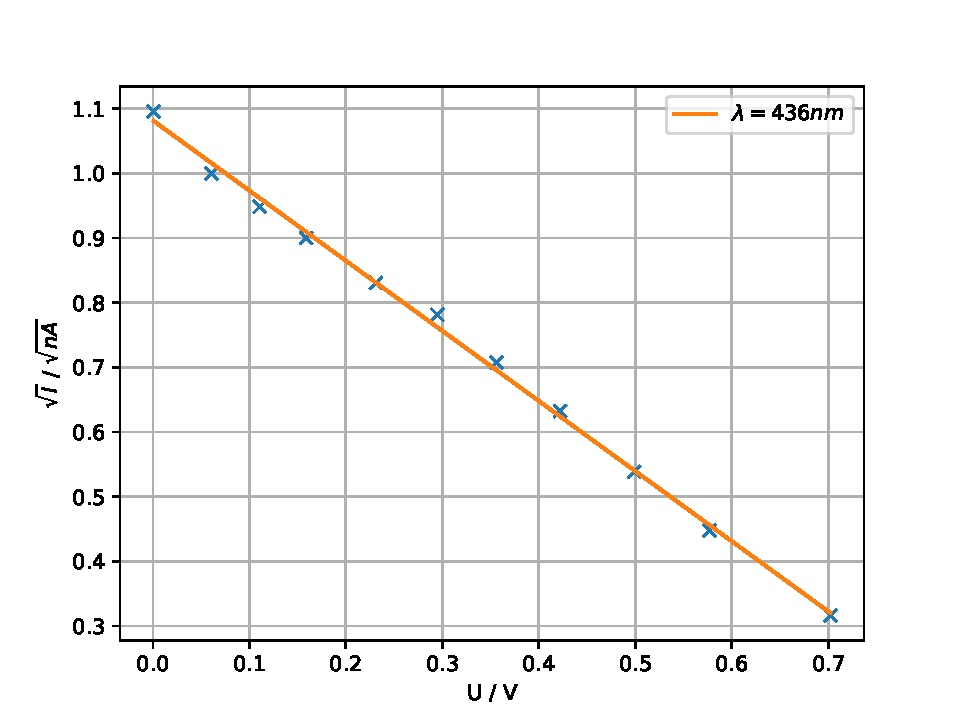
\includegraphics[width=\textwidth]{Violett436.pdf}
  \caption{Photostrom $I$ gegen Bremsspannung $U$ für $\lambda=436nm$ (Violett)}
  \label{fig:v436}
\end{figure}
\FloatBarrier
\begin{align*}
  c &= (-3,429 \pm 9,474 \cdot 10^{-9}) 10^{-5}\si{\frac{\sqrt{A}}{V}}\\
  d &= (3,421 \pm 4,333 \cdot 10^{-9}) 10^{-5}\si{\sqrt{A}}\\
  -\frac{d}{c} &= \SI{0.998}{V}
\end{align*}
\FloatBarrier
\begin{table}[h!]
  \centering
  \caption{Photostrom $I$ in Abhängigkeit von der Bremsspannung $U$ für $\lambda=\SI{492}{nm}$}
  \label{tab:g492}
  \begin{tabular}{c c c}
    \toprule
      U/V & I/nA  & $\sqrt{I}$/$\sqrt{nA}$ \\
    \midrule
      0,001 & 0,082 & 0,286 \\
      0,069 & 0,070 & 0,265 \\
      0,131 & 0,060 & 0,245 \\
      0,182 & 0,050 & 0,224 \\
      0,246 & 0,040 & 0,200 \\
      0,305 & 0,030 & 0,173 \\
      0,379 & 0,020 & 0,141 \\
      0,486 & 0,010 & 0,100 \\
      0,763 & 0,000 & 0,000 \\


    \bottomrule
  \end{tabular}
\end{table}

\FloatBarrier
\begin{figure}[h!]
  \centering
  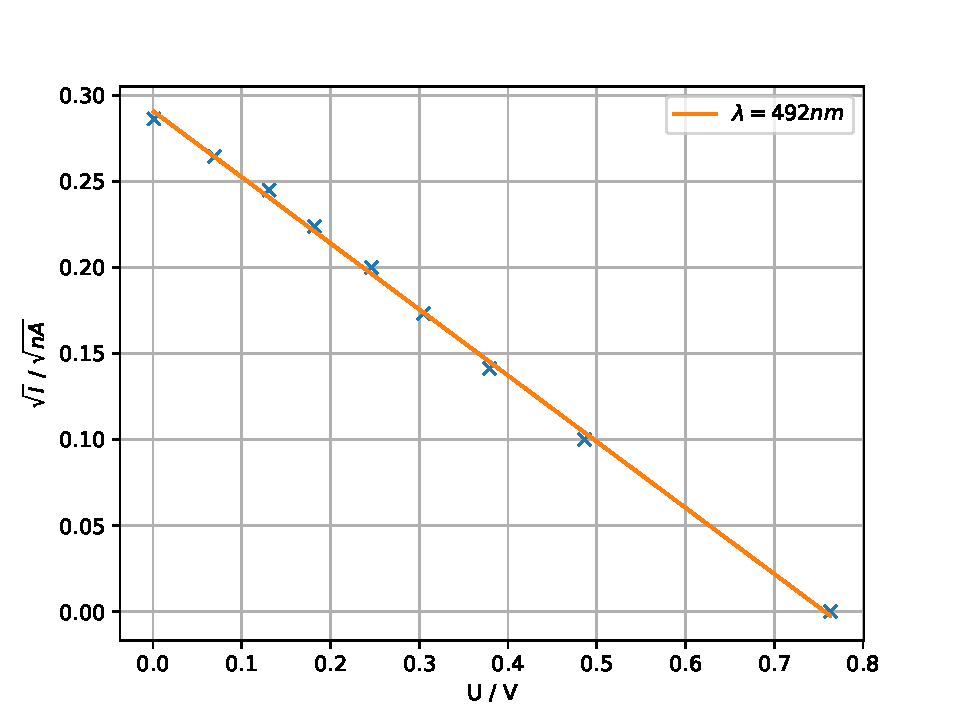
\includegraphics[width=\textwidth]{Cyan492.pdf}
  \caption{Photostrom $I$ gegen Bremsspannung $U$ für $\lambda=492nm$ (Cyan)}
  \label{fig:g492}
\end{figure}
\FloatBarrier
\begin{align*}
  e &= (-1,216 \pm 3,049 \cdot 10^{-9}) 10^{-5}\si{\frac{\sqrt{A}}{V}}\\
  f &= (9,202 \pm 3,966 \cdot 10^{-9}) 10^{-6}\si{\sqrt{A}}\\
  -\frac{f}{e} &= \SI{0.757}{V}
\end{align*}
\FloatBarrier
\begin{table}[h!]
  \centering
  \caption{Photostrom $I$ in Abhängigkeit von der Bremsspannung $U$ für $\lambda=\SI{546}{nm}$}
  \label{tab:g546}
  \begin{tabular}{c c c}
    \toprule
      U/V & I/nA  & $\sqrt{I}$/$\sqrt{nA}$  \\
    \midrule
      0,001 & 0,61 & 0,781 \\
      0,113 & 0,50 & 0,707 \\
      0,195 & 0,40 & 0,632 \\
      0,275 & 0,30 & 0,548 \\
      0,353 & 0,20 & 0,447 \\
      0,443 & 0,10 & 0,316 \\
      0,458 & 0,08 & 0,283 \\
      0,490 & 0,06 & 0,245 \\
      0,529 & 0,04 & 0,200 \\
      0,590 & 0,02 & 0,141 \\


    \bottomrule
  \end{tabular}
\end{table}

\FloatBarrier
\begin{figure}[h!]
  \centering
  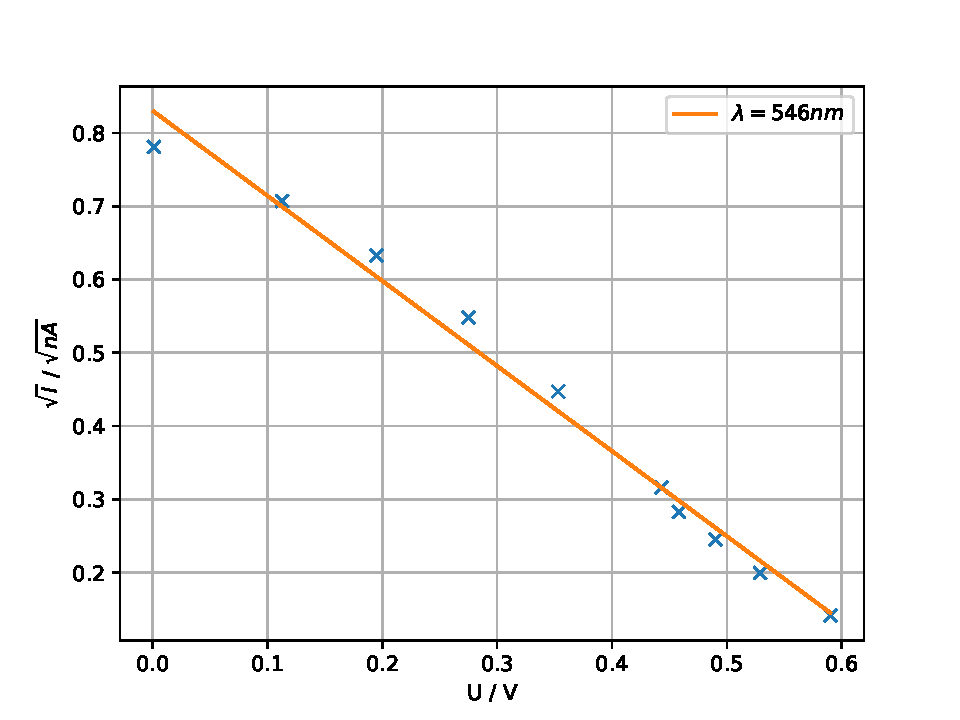
\includegraphics[width=\textwidth]{Gruen546.pdf}
  \caption{Photostrom $I$ gegen Bremsspannung $U$ für $\lambda=546nm$ (Grün)}
  \label{fig:g546}
\end{figure}
\FloatBarrier
\begin{align*}
  g &= (-3,671 \pm 2,245 \cdot 10^{-7}) 10^{-5}\si{\frac{\sqrt{A}}{V}}\\
  h &= (2,626 \pm 3,423 \cdot 10^{-8}) 10^{-5}\si{\sqrt{A}}\\
  -\frac{h}{g} &= \SI{0.715}{V}
\end{align*}
\FloatBarrier
\begin{table}[h!]
  \centering
  \caption{Photostrom $I$ in Abhängigkeit von der Bremsspannung $U$ für $\lambda=\SI{578}{nm}$}
  \label{tab:o578}
  \begin{tabular}{c c c}
    \midrule
      U/V & I/nA  & $\sqrt{I}$/$\sqrt{nA}$ \\
    \midrule
      0,001 & 0,30 & 0,548\\
      0,148 & 0,20 & 0,447\\
      0,289 & 0,10 & 0,316\\
      0,308 & 0,08 & 0,283\\
      0,316 & 0,07 & 0,265\\
      0,335 & 0,06 & 0,245\\
      0,356 & 0,05 & 0,224\\
      0,379 & 0,04 & 0,200\\
      0,399 & 0,03 & 0,173\\
      0,437 & 0,02 & 0,141\\
      0,479 & 0,01 & 0,100\\
      0,545 & 0,00 & 0,000\\


    \bottomrule
  \end{tabular}
\end{table}

\FloatBarrier
\begin{figure}[h!]
  \centering
  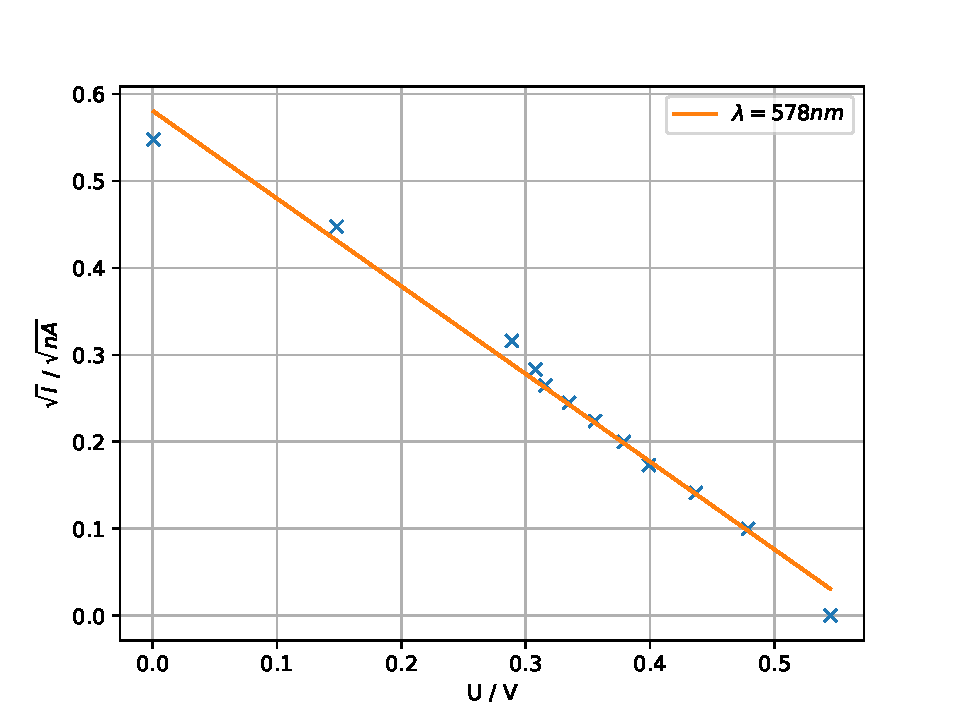
\includegraphics[width=\textwidth]{Orange578.pdf}
  \caption{Photostrom $I$ gegen Bremsspannung $U$ für $\lambda=578nm$ (Orange)}
  \label{fig:o578}
\end{figure}
\FloatBarrier
\begin{align*}
  i &= (-3,191 \pm  1,373 \cdot 10{-7}) 10^{-5}\si{\frac{\sqrt{A}}{V}}\\
  j &= (1,837 \pm 1,785 \cdot 10^{-8}) 10^{-5}\si{\sqrt{A}}\\
  -\frac{j}{i} &= \SI{0.576}{V}
\end{align*}
\FloatBarrier
Die Frequenz des Lichtes berechnet sich aus der Wellenlänge $\lambda$ und der Lichtgeschwindigkeit c:
\begin{equation*}
  f=\frac{c}{\lambda}.
\end{equation*}
\\Die Grenzspannungen $U_g$ werden gegen die Lichtfrequenz aufgetragen (Tab. \ref{tab:hdurchenull}, Abb. \ref{fig:hdurchenull}).
Die lineare Ausgleichsrechnung der Form $y=kx+l$ wird mit Python gemacht.
\begin{table}[h!]
  \centering
  \caption{Bremsspannung $U_g$ in Abhängigkeit von der Wellenlänge $\lambda$ bzw. der Frequenz $f$}
  \label{tab:hdurchenull}
  \begin{tabular}{c c c}
    \toprule
      $\lambda$ & f  & $U_g$ \\
      nm        & $10^{15}$Hz & V \\
    \midrule
    405 & 0,7402 & 1,151 \\
    436 & 0,6876 & 0,998 \\
    492 & 0,6093 & 0,757 \\
    546 & 0,5491 & 0,715 \\
    578 & 0,5187 & 0,576 \\






    \bottomrule
  \end{tabular}
\end{table}

\begin{figure}[h!]
  \centering
  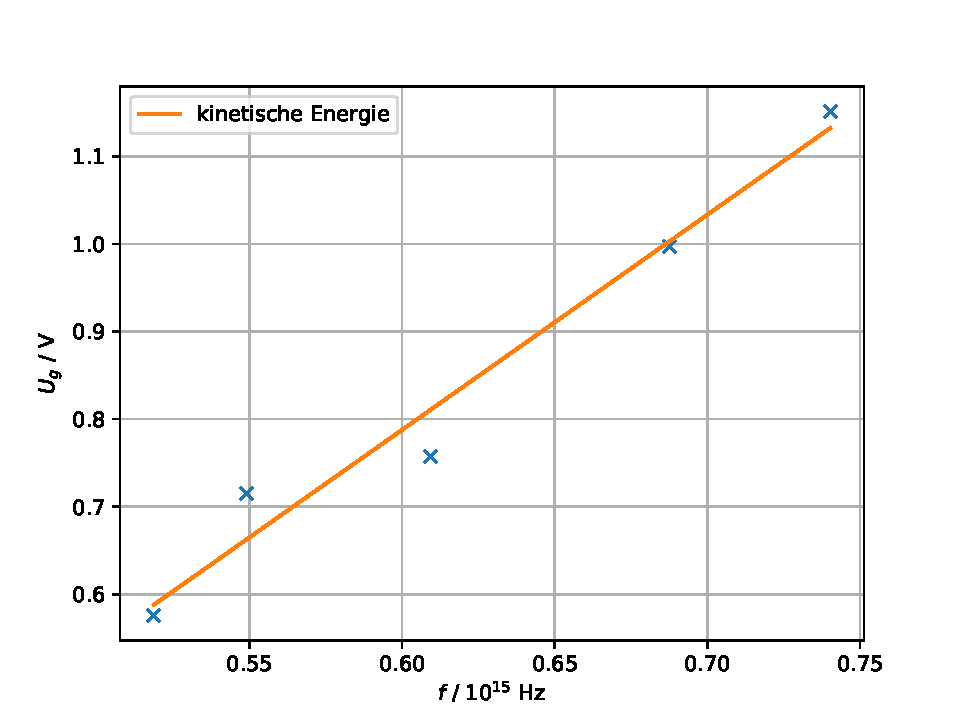
\includegraphics[width=\textwidth]{hdurchenull.pdf}
  \caption{Grenzspannung gegen Lichtfrequenz}
  \label{fig:hdurchenull}
\end{figure}
Um die Größe $h/e_0$ zu bestimmen wird die kinetische Energie der Elektronen wie folgt umgestellt:
\begin{equation*}
  h f = e_0 U_g + A_K \Leftrightarrow
  U_g = \frac{h}{e_0} f -\frac{A_K}{e_0}.
\end{equation*}
Die Steigung $k$ des Graphen in Abbildung \ref{fig:hdurchenull} entspricht der Größe $h/e_0$, der Y-Achsenabschnitt $l$ entpricht der Größe $-A_K/e_0$:
\begin{align*}
  \frac{h}{e_0} =& k =& \SI{2.457 \pm 0.060} 10^{-15}\si{\frac{A}{V}}\\
  \frac{A_K}{e_0} =& l =& \SI{-0.687 \pm 0.024}{V}
\end{align*}
$l$ mit der Elektronenladung \cite{taschenrechner} multipliziert ergibt die Austrittsarbeit $A_K$:
\begin{equation*}
  A_K=\SI{1.1002 \pm 0.0038}{10^{-19}} \si{J} = \SI{0.687 \pm 0.024}{eV}
\end{equation*}
\FloatBarrier
\subsection{Abhängigkeit des Elektronenstroms von der Gegenspannung}
Die Messwerte des Photostrom und der Gegenspannung sind in Tabelle \ref{tab:messreihe2} notiert.
Die Abbildung \ref{fig:Messreihe2} zeigt den Stromverlauf in Abhängigkeit der Gegenspannung.
\begin{table}[h!]
  \centering
  \caption{Photostrom $I$ in Abhängigkeit von der Bremsspannung $U$ für $\lambda=\SI{578}{nm}$}
  \label{tab:messreihe2}
  \begin{tabular}{c c c c}
    \toprule
      U/V & I/nA  & U/V & I/nA\\
    \midrule
     0,001 & 0,30 & -1,236 & 0,70 \\
     0,148 & 0,20 & -1,600 & 0,80 \\
     0,289 & 0,10 & -1,855 & 0,90 \\
     0,308 & 0,08 & -2,32  & 1,00 \\
     0,316 & 0,07 & -3,67  & 1,20 \\
     0,335 & 0,06 & -3,67  & 1,40 \\
     0,356 & 0,05 & -3,94  & 1,50 \\
     0,379 & 0,04 & -4,24  & 1,60 \\
     0,399 & 0,03 & -6,31  & 1,70 \\
     0,437 & 0,02 & -8,05  & 1,80 \\
     0,479 & 0,01 & -9,75  & 1,90 \\
     0,545 & 0,00 & -7,41  & 2,00 \\
    -0,001 & 0,28 & -10,50 & 2,20 \\
    -0,272 & 0,40 & -12,98 & 2,40 \\
    -0,554 & 0,50 & -19,16 & 2,50 \\
    -0,898 & 0,60 & -16,33 & 2,60 \\

    \bottomrule
  \end{tabular}
\end{table}

\begin{figure}[h!]
  \centering
  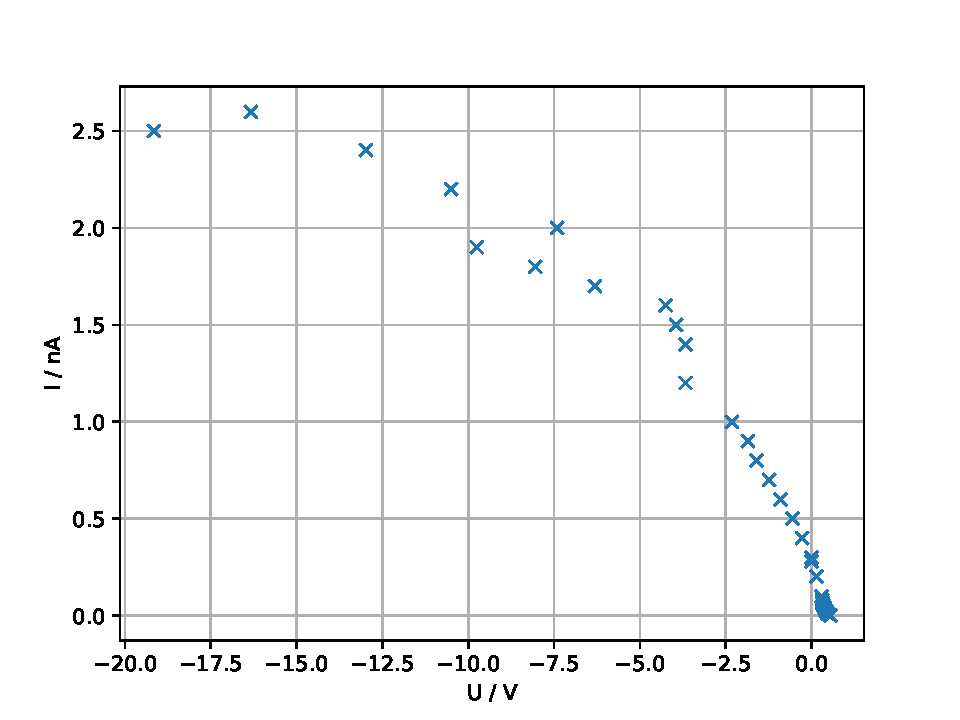
\includegraphics[width=\textwidth]{messreihe2.pdf}
  \caption{Photostrom gegen Gegenspannung}
  \label{fig:Messreihe2}
\end{figure}
\FloatBarrier
